%\newcommand{\ein}[2]{(#1) (#2 Punkte)}


\begin{Large}
\textbf{Teil I: Offene Aufgaben (36 Punkte)}
\end{Large}
\\
\\
\\
\textbf{Allgemeine Anweisungen für offene Fragen:}
\\
\renewcommand{\labelenumi}{(\roman{enumi})}
\begin{enumerate}
\item
Ihre Antworten müssen alle Rechenschritte enthalten,
diese müssen klar ersichtlich sein.
Verwendung korrekter mathematischer Notation wird erwartet
und fliesst in die Bewertung ein.

\item
Ihre Antworten zu den jeweiligen Teilaufgaben müssen in den dafür vorgesehenen Platz geschrie-
ben werden. Sollte dieser Platz nicht ausreichen, setzen Sie Ihre Antwort auf der Rückseite oder
dem separat zur Verfügung gestellten Papier fort. Verweisen Sie in solchen Fällen ausdrücklich
auf Ihre Fortsetzung. Bitte schreiben Sie zudem Ihren Vor- und Nachnamen auf jeden separaten
Lösungsbogen.

\item
Es werden nur Antworten im dafür vorgesehenen Platz bewertet. Antworten auf der Rückseite
oder separatem Papier werden nur bei einem vorhandenen und klaren Verweis darauf bewertet.

\item
Die Teilaufgaben werden mit den jeweils oben auf der Seite angegebenen Punkten bewertet.

\item
Ihre endgültige Lösung jeder Teilaufgabe darf nur eine einzige Version enthalten.

\item
Zwischenrechnungen und Notizen müssen auf einem getrennten Blatt gemacht werden. Diese
Blätter müssen, deutlich als Entwurf gekennzeichnet, ebenfalls abgegeben werden.
\end{enumerate}

\newpage
\section*{\hfil Aufgaben \hfil}
\vspace{1cm}
\section*{Aufgabe 1 (36 Punkte)}
\vspace{0.4cm}
%\titleformat{\subsection}[runin]
%{\normalfont\large\bfseries}{\thesubsection}{1em}{}
\subsection*{\aufgabe{a1}{6}} 
Thomas Robert Malthus (1766-1834), ein britischer Ökonom und Pfarrer, veröffentlichte
1798 seinen vielbeachteten \textit{Essay on the Principle of Population}.
Er formulierte das Axiom, dass die Weltbevölkerung exponentiell wachse, die Nahrung dagegen nur linear. 
Das bedeutet, dass die Funktion $ n(t) $, welche die Anzahl Menschen angibt, die man bei optimaler Verteilung der zur Verfügung stehenden Nahrungsmittel zu Zeit $ t $ ernähren könnte, eine lineare ist:
\begin{align*}
	n(t) = a + b \cdot t.
\end{align*}
Die Weltbevölkerung $ w(t) $ betrug im Jahre 1800 ($ t= 0 $) rund eine Milliarde, d.h. $ w(0) = 10^9 $.
Wir wollen annehmen, dass die Weltbevölkerung rund $ 1\% $ pro Jahr wächst.
Außerdem wollen wir mit
\begin{align*}
	a = 2 \cdot 10^9 \ \textrm{und} \ b = 0.2 \cdot 10^9
\end{align*}
rechnen.
\begin{description}
	\item[Beweisen Sie:] 
	Es gibt genau einen Zeitpunkt $ t^\star > 400 $, an dem die Weltbevölkerung gerade noch ernährt werden kann, d.h., für $ w(t^\star)  = n(t^\star )$ ist.
\end{description}  
\
\\


\subsection*{\aufgabe{a2}{6}}
Thomas Robert Malthus (1766-1834), ein britischer Ökonom und Pfarrer, veröffentlichte
1798 seinen vielbeachteten \textit{Essay on the Principle of Population}.
Er formulierte das Axiom, dass die Weltbevölkerung exponentiell wachse, die Nahrung dagegen nur linear. 
Das bedeutet, dass die Funktion $ n(t) $, welche die Anzahl Menschen angibt, die man bei optimaler Verteilung der zur Verfügung stehenden Nahrungsmittel zu Zeit $ t $ ernähren könnte, eine lineare ist:
\begin{align*}
	n(t) = a + b \cdot t.
\end{align*}
Die Weltbevölkerung $ w(t) $ betrug im Jahre 1800 ($ t= 0 $) rund eine Milliarde, d.h. $ w(0) = 10^9 $.
Wir wollen annehmen, dass die Weltbevölkerung rund $ 1\% $ pro Jahr wächst.
Außerdem wollen wir mit
\begin{align*}
	a = 2 \cdot 10^9 \ \textrm{und} \ b = 0.2 \cdot 10^9
\end{align*}
rechnen.\\
\\
Es gibt genau einen Zeitpunkt $ t^\star > 400 $, an dem die Weltbevölkerung gerade noch ernährt werden kann, d.h., für $ w(t^\star)  = n(t^\star )$ ist.\\
\\
Verwenden Sie eine Taylor-Approximation zweiter Ordnung im Punkt $ t_0 = 400 $, um eine Näherung für $ t^\star $ zu finden.
 \\
\\
\titleformat{\subsection}[display]
{\normalfont\large\bfseries}{\thesubsection}{1mm}{}
\subsection*{\aufgabe{b}{10}}
Max hat über seine Verhältnisse gelebt. 
Deshalb hat er nun Schulden von mehreren hunderttausend Franken.
Die Schuldenberatung vermittelt ihm am Anfang des Jahres einen Privatkredit mit $ i = 5 \% $ in der genannten Höhe von $ S = 355'000 \ [\textrm{CHF}] $, den er in $ 12 $ gleich grossen Raten $ C $ jeweils per Jahresende abbezahlen muss. 
\begin{enumerate}
	\item[(b1)] Fügen Sie die Ereignisse und Mittelflüsse dem Zeitstrahl hinzu.
	\item[(b2)] Berechnen Sie die Höhe der Ratenzahlung $ C $.
\end{enumerate}
Am Ende des vierten Jahres gewinnt Max im Lotto CHF $ 160'000 $.
Er beschließt in diesem Jahr statt der normalen Rate $ C $ den ganzen Lottogewinn zur Abzahlung des Kredits zu benützen.
\begin{enumerate}
	\item[(b3)] Ergänzen Sie die Information am Zeitstrahl und berechnen Sie die Restschuld $ \overline{S} $ nach der Einzahlung am Ende des vierten Jahres.
\end{enumerate}
Max zahlt nun weiter am Ende jeden Jahres den Betrag $ C $ zu Tilgung seiner Restschuld $ \overline{S} $.
\begin{enumerate}
	\item[(b4)] Wie viele Zahlungen muss er machen, bis er die Restschuld vollkommen getilgt hat?
	\item[(b5)] Mit der letzten Rate muss nicht mehr der komplette Betrag $ C $ geleistet werden. Wie hoch ist die Zahlung genau?
\end{enumerate}
\begin{center}
	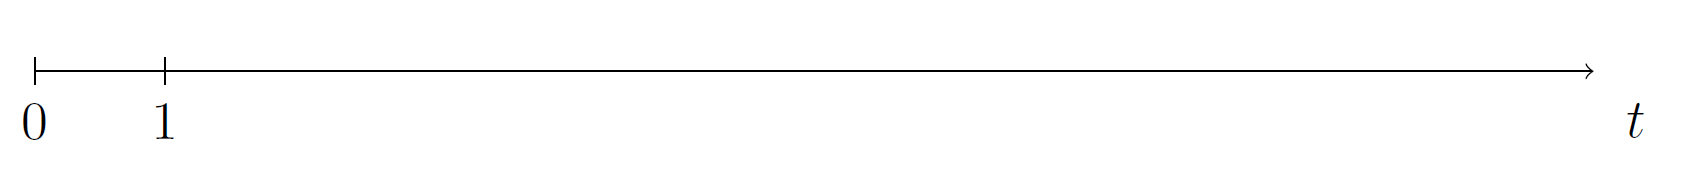
\includegraphics[scale=0.3]{pictures/zeitstrahl_1_b}
\end{center}
\ \\
\subsection*{\aufgabe{c}{6}}
Nach der Relativitätstheorie gilt für die Masse $ m $ eines Körpers, der sich mit der Geschwindigkeit $ v $ bewegt
\begin{align*}
	m(v)
	=
	\frac{m_0}{\sqrt{1 - \frac{v^2}{c^2}}}.
\end{align*}
Dabei ist $ c $ die Lichtgeschwindigkeit $ (299'792'458 \nicefrac{m}{s}) $ und $ m_0 $ die Masse in Ruhe.
\begin{enumerate}
	\item[(c1)] Berechnen Sie die Elastizität $ \varepsilon_m $ von $ m(v) $.
	\item[(c2)] Um wie viel Prozent ändert sich näherungsweise die Masse, wenn die Geschwindigkeit von $ v_0 = 0.5c $ um $ 5 \% $ erhöht wird?
\end{enumerate}
\
\\
\subsection*{\aufgabe{d}{8}}
Bei einer Absatzmenge $ x \geq 20  $ kann ein Monopolist mit dem Ertrag $ E(x) $ und den Kosten $ K(x) $ rechnen, die wie folgt gegeben sind:
\begin{align*}
	E(x) = -0.5 x^{1.5} +100 x \ \textrm{und} \ K(x) = -200\sqrt{x} + 50 x +120.
\end{align*}
Von seinem Bruttogewinn muss der Hersteller $ i \% $  $ (0 < i < 100) $ an Steuern bezahlen.
\begin{enumerate}
	\item[(d1)]
	Drücken Sie den Gewinn $ G(x) $ nach Steuern in Abhängigkeit der verkauften Menge $ x $ aus.
	\item[(d2)] 
	Für welche Menge $ x^\star $ maximiert der Hersteller seinen Gewinn nach Steuern?
\end{enumerate}


\newpage


\fancyhead[C]{\normalsize\textbf{$\qquad$ Teil II: Multiple-Choice}}
\begin{Large}
\textbf{Teil II: Multiple-Choice-Fragen (64 Punkte)}
\end{Large}
\\
\\
\\
\textbf{Allgemeine Anweisungen für Multiple-Choice-Fragen:}
\\
\renewcommand{\labelenumi}{(\roman{enumi})}
\begin{enumerate}
\item
Die Antworten auf die Multiple-Choice-Fragen müssen im dafür vorgesehenen Antwortbogen ein-
getragen werden. Es werden ausschliesslich Antworten auf diesem Antwortbogen bewertet. Der
Platz unter den Fragen ist nur für Notizen vorgesehen und wird nicht korrigiert.

\item
Jede Frage hat nur eine richtige Antwort. Es muss also auch jeweils nur eine Antwort angekreuzt werden.

\item
Falls mehrere Antworten angekreuzt sind, wird die Antwort mit 0 Punkten bewertet, auch wenn
die korrekte Antwort unter den angekreuzten ist.

\item
Bitte lesen Sie die Fragen und die Anweisungen auf dem Multiple-Choice-Antwortbogen sorgfältig.

\end{enumerate}
\newpage
\section*{Aufgabe 2 (34 Punkte)}
\vspace{0.4cm}

\subsection*{\frage{1}{3}}
$ A $ und $ B $ seien zwei Aussagen. Die zusammengesetzte Aussage
\begin{align*}
	\neg (A \ \Rightarrow \ \neg B)
\end{align*}
ist äquivalent zu 
 \renewcommand{\labelenumi}{(\alph{enumi})}
\begin{enumerate}
\item $ A \vee B $.
\item $ A \wedge B $.
\item $ (\neg A) \vee (\neg B)$
\item $ (\neg A) \wedge (\neg B)$.
\end{enumerate}
\ \\
\subsection*{\frage{2}{2}}
Die Folge $ \lbrace a_n \rbrace_{n \in \N} $ ist monoton wachsend und konvergiert mit $ \lim_{n \to \infty} a_n = -2 $.
Die Folge $ \lbrace b_n \rbrace_{n \in \N} $ ist definiert durch $ b_n = (-3) \cdot a_n $.\\
\\
Dann folgt:
\renewcommand{\labelenumi}{(\alph{enumi})}
\begin{enumerate}
\item $ \lbrace b_n \rbrace_{n \in \N} $ ist monoton wachsend und divergent.
\item $ \lbrace b_n \rbrace_{n \in \N} $ ist monoton wachsend und konvergent.
\item $ \lbrace b_n \rbrace_{n \in \N} $ ist monoton fallend und divergent.
\item $ \lbrace b_n \rbrace_{n \in \N} $ ist monoton fallend und konvergent.
\item $ \lbrace b_n \rbrace_{n \in \N} $ ist nicht monoton und divergent.
\end{enumerate}
\ \\
\subsection*{\frage{3}{3}}
Eine Möbelfirma wirbt:
\begin{center}
	\glqq Wir schenken Ihnen die Mehrwertsteuer auf Ihren Möbelkauf\grqq
\end{center}
Die Mehrwertsteuer auf Möbel beträgt in der Schweiz $ 7.7 \% $.\\
Wie viel Prozent Rabatt gewährt also die Möbelfirma?
\renewcommand{\labelenumi}{(\alph{enumi})}
\begin{enumerate}
\item 
Es sind etwa $ 7.15 \% $.
\item 
Es sind etwa $ 7.56 \% $.
\item 
Es sind genau $ 7.7 \% $.
\item
Es sind etwa $ 7.78 \% $.
\item
Es sind etwa $ 8.34 \% $.
\end{enumerate}
\ \\
\subsection*{\frage{4}{3}}
Sei $ f $ eine Funktion einer reellen Variablen und $ x_0 \in D_f $.
$ x_0  $ heißt \textit{Fixpunkt von} $ f $, wenn gilt: $ f(x_0) = x_0 $.\\
\\
Welche der folgenden Aussagen ist wahr? 
\renewcommand{\labelenumi}{(\alph{enumi})}
\begin{enumerate}
	\item 
	Wenn $ f $ invertierbar ist, dann hat $ f $ keinen Fixpunkt.
	\item
	Wenn $ f $ invertierbar ist und $ f^{-1} $ mehrere Fixpunkte hat, dann hat $ f $ höchstens einen Fixpunkt.
	\item
	Wenn $ f $ invertierbar ist, dann hat $ f $ mindestens einen Fixpunkt.
	\item
	Wenn $ f  $ einen Fixpunkt hat, dann ist $ f $ invertierbar.
	\item
	Wenn $ f $ invertierbar ist und einen Fixpunkt hat, dann hat auch $ f^{-1} $ einen Fixpunkt.
\end{enumerate}
\ \\
\subsection*{\frage{5}{3}}
Seien $ a,b >0, \ b \neq 1 , \ n \in \N  $.\\
Welche der folgenden Identitäten ist allgemein gültig?
\renewcommand{\labelenumi}{(\alph{enumi})}
\begin{enumerate}
	\item 
	$ \log_{b^n}(a^n) = \frac{\log_{b}(a)}{n} $.
	\item 
	$ \log_{b^n}(a^n) = \sqrt[n]{\log_{b}(a)} $.
	\item
	$ \log_{b^n}(a^n) = \log_{b}(a) $.
	\item
	$ \log_{b^n}(a^n) = n \ \log_{b}(a) $.
	\item
	Keine der vorangehenden Aussagen ist im Allgemeinen gültig.
\end{enumerate}
\ \\
\subsection*{\frage{6}{3}}
Ein Bergsteiger startet bei seinem Auto bei Sonnenaufgang um $ 5 $ Uhr mit dem Aufstieg und erreicht auf direktem Weg ohne Pause die Hütte um $ 13 $ Uhr.
Am anderen Tag geht er den genau gleichen Weg zurück; er startet um $ 8 $ Uhr und geht ohne anzuhalten. So erreicht er sein Auto um $12$:$50$  Uhr.\\
\\
Gibt es einen Tageszeitpunkt, zu dem er auf dem Weg aufwärts bzw. auf dem Weg abwärts an der gleichen Stelle ist? 
\renewcommand{\labelenumi}{(\alph{enumi})}
\begin{enumerate}
	\item 
	Ja, es gibt genau einen solchen Zeitpunkt.
	\item 
	Nein.
	\item
	Es kann sein, muss aber nicht sein.
	\item
	Es kann auch mehrere Zeitpunkte geben.
\end{enumerate}
\ \\
\subsection*{\frage{7}{3}}
Gegeben ist die Funktion $ f $ definiert durch
\begin{align*}
	f(x) = \sin(x) + \cos(x)
\end{align*}
mit Definitionsgebiet $ D_f \in \R $. Für den Wertebereich $ W_f $ von $ f $ gilt:
\renewcommand{\labelenumi}{(\alph{enumi})}
\begin{enumerate}
\item 
$ W_f = [-1,1] $.
\item
$ W_f = [-\sqrt{2},\sqrt{2}] $.
\item
$ W_f = [-2,2] $.
\item
$ W_f = [0,2] $.
\item
$ W_f = [-\nicefrac{\pi }{2}, \nicefrac{\pi }{2}] $.
\end{enumerate}
\ \\
\subsection*{\frage{8}{3}}
$ f $ und $ g $ seien ungerade, differenzierbare Funktionen. Dann gilt:
\renewcommand{\labelenumi}{(\alph{enumi})}
\begin{enumerate}
	\item 
	$ f^\prime + g^\prime $ ist ungerade.
	\item
	$ f^\prime + g^\prime $ ist gerade.
	\item
	$ f^\prime \cdot g^\prime $ ist ungerade.
	\item
	Keine der obigen Antworten ist im Allgemeinen richtig.
\end{enumerate}
\ \\
\subsection*{\frage{9}{2}}
Wir betrachten die differenzierbaren Funktionen $ f(x) $ und $ g(x) $, wobei $ g(x) > 0 $ für $ x \in \R $ gelte. Die Ableitung der Funktion
\begin{align*}
	k(x)
	=
	\frac{f(g(x))}{g(f(x))}
\end{align*}
ist dann
\renewcommand{\labelenumi}{(\alph{enumi})}
\begin{enumerate}
	\item 
	$ k^\prime(x) = \frac{f^\prime(g(x))g(f(x)) + f(g(x))g^\prime(f(x))}{(g(f(x)))^2} $.
	\item
	$ k^\prime(x) = \frac{f^\prime(g(x))g^\prime(x) }{g^\prime(f(x))f^\prime(x)} $.
	
	\item
    $ k^\prime(x) = 
    \frac{f^\prime(g(x))g^\prime(x)g(f(x)) - f(g(x)) g^\prime(f(x)) f^\prime(x) }
    {(g(f(x)))^2} $.
	\item
	$ k^\prime(x) = \frac{f^\prime(g(x))g(f(x)) - f(g(x))g^\prime(f(x))}{(g(f(x)))^2} $.
\end{enumerate}
\ \\
\subsection*{\frage{10}{3}}
Gegeben ist die Funktion
\begin{align*}
	f \ : \ \R \rightarrow \R, \ x \mapsto y = x \cdot |x| 
\end{align*}
Dann folgt:
\renewcommand{\labelenumi}{(\alph{enumi})}
\begin{enumerate}
	\item 
	$ f $ ist überall stetig und differenzierbar.
	\item
	$ f $ ist stetig in $ x_0 = 0 $, aber nicht differenzierbar in $ x_0 = 0 $.
	\item
	$ f $ ist differenzierbar in $ x_0 = 0 $, aber nicht stetig in $ x_0 = 0 $.
	\item
	$ f $ ist nicht stetig und nicht differenzierbar in $ x_0 = 0 $.
\end{enumerate}
\ \\
\subsection*{\frage{11}{3}}
Das Taylorpolynom $ 4 $. Ordnung in $ x_0 = 0 $ der Funktion
\begin{align*}
	f(x) = e^{x^3}
\end{align*}
lautet:
\renewcommand{\labelenumi}{(\alph{enumi})}
\begin{enumerate}
	\item 
	$ P_4(x) = \frac{x^4}{4} + \frac{x^3}{3} + \frac{x^2}{2} + x $. 
	\item
	$ P_4(x) = \frac{x^4}{4} + \frac{x^3}{3} + \frac{x^2}{2} - x $. 
	\item
	$ P_4(x) = x^3 + x^2 + x + 2$. 
	\item
	$ P_4(x) = \frac{x^4}{4} + \frac{x^3}{3} + \frac{x^2}{2} + x +1 $. 
	\item
	$ P_4(x) = x^3 + 1$. 
	\item
	$ P_4(x) = \frac{x^4}{4} - \frac{x^3}{3} + \frac{x^2}{2} - x + 2 $. 
\end{enumerate}
\ \\
\subsection*{\frage{12}{3}}
Die Funktion zweier Variablen $ f $ ist homogen vom Grad $ 3 $ und die Funktion zweier Variablen $ g $ ist homogen vom Grade $ -3 $.\\
\\
Die Funktion $ h $ ist definiert durch
\begin{align*}
	h(x,y) = f(g(x,y),g(x,y)).
\end{align*}
Dann gilt:
\renewcommand{\labelenumi}{(\alph{enumi})}
\begin{enumerate}
	\item 
	$ h $ ist homogen vom Grad $ -1 $. 
	\item
	$ h $ ist homogen vom Grad $ 0 $. 
	\item
	$ h $ ist homogen vom Grad $ 6 $. 
	\item
	$ h $ ist homogen vom Grad $ -9 $.  
	\item
	$ h $ ist nicht homogen.
\end{enumerate}

\newpage
\section*{Aufgabe 3 (30 Punkte)}
\vspace{0.4cm}

\subsection*{\frage{1}{4}}
Es sei
\begin{align*}
	s = \sum \limits_{i= 1}^3
	\sum \limits_{j= 1}^2
	\sum \limits_{k= 1}^4
	(i + jk).
\end{align*}
Dann gilt:
\renewcommand{\labelenumi}{(\alph{enumi})}
\begin{enumerate}
	\item 
	$ s= 138 $.
	\item
	$ s= 144 $.
	\item
	$ s= 132 $.
	\item
	$ s= 180 $.
	\item
	$ s= 120 $.
	\item
	$ s= 128 $.
\end{enumerate}
\ \\
\subsection*{\frage{2}{4}}
Der Grenzwert
\begin{align*}
	\lim\limits_{x \to 0 }
	\frac{\sqrt[n]{a+x} - \sqrt[n]{a-x}}{x}
\end{align*}
für einen fest gewählten Parameter $ a > 0  $ ist gleich:
\renewcommand{\labelenumi}{(\alph{enumi})}
\begin{enumerate}
	\item 
	$0$.
	\item
	$1$.
	\item
	$\frac{\sqrt[n]{a}}{na}$.
	\item
	$\frac{2}{n} \sqrt[n]{a}$.
	\item
	$\frac{2}{n} \sqrt[n]{a^{1-n}}$.
	\item
	Der obige Ausdruck hat für $ x \to 0 $ keinen Grenzwert.	
\end{enumerate}
\ \\
\subsection*{\frage{3}{4}}
Gegeben ist die Funktion
\begin{align*}
	f(x) = x^{\ln(x)}.
\end{align*}
Welcher der folgenden Ausdrücke beschreibt die erste Ableitung von $ f $ ?
\renewcommand{\labelenumi}{(\alph{enumi})}
\begin{enumerate}
\item 
$ f^\prime(x) = [\ln(x)]^2 x^{\ln(x)} \frac{1}{x}$.
\item
$ f^\prime(x) =2 x^{\ln(x) -1} \ln(x) $.
\item
$ f^\prime(x) = \ln(x) x^{\ln(x) -1} $.
\item
$ f^\prime(x) =  x^{\ln(x) }\ln(x)\frac{1}{x} $.
\item
Keine der vorangehenden Formeln für $ f^\prime(x)  $ ist korrekt.
\end{enumerate}
\ \\
\subsection*{\frage{4}{4}}
Gegeben ist die Funktion $ f $ zweier reeller Variablen
\begin{align*}
	f \ : \ D_f \to \R, \ (x,y) \mapsto z = f(x,y) =\sqrt{(36 - x^2 -y^2) y}.
\end{align*}
Welches der folgenden Bilder zeigt grau schraffiert den Definitionsbereich $ D_f \subset \R^2 $ von $ f $?
\renewcommand{\labelenumi}{(\alph{enumi})}
\begin{enumerate}
\item 
\begin{center}
	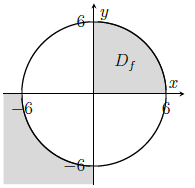
\includegraphics[scale=0.6]{pictures/3_4_a}
\end{center}
\item 
\begin{center}
	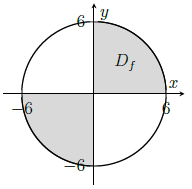
\includegraphics[scale=0.6]{pictures/3_4_b}
\end{center}
\item
\begin{center}
	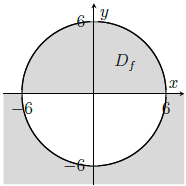
\includegraphics[scale=0.6]{pictures/3_4_c}
\end{center}
\item
\begin{center}
	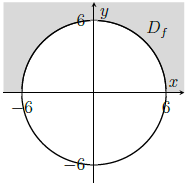
\includegraphics[scale=0.6]{pictures/3_4_d}
\end{center}
\end{enumerate}
\ 
\subsection*{\frage{5}{3}}
Welche der folgenden Funktionen gehört zur unten dargestellten Fläche?\\
\begin{center}
	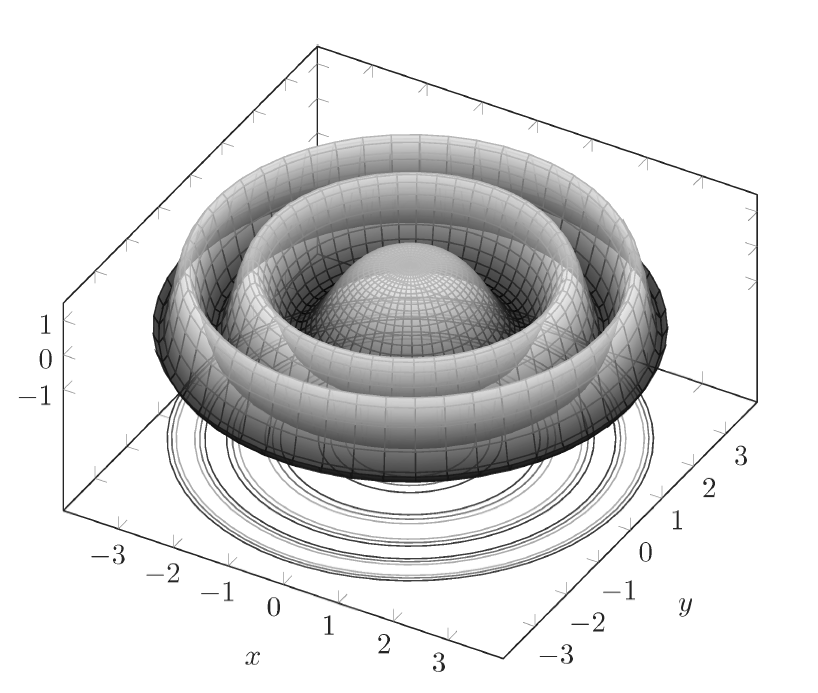
\includegraphics[scale=0.5]{pictures/3_5}
\end{center}
\renewcommand{\labelenumi}{(\alph{enumi})}
\begin{enumerate}
\item 
$ z = f_1(x,y) = e^{-(x+y^2)} $.
\item
$ z = f_2(x,y) = e^{x} e^y $.
\item
$ z = f_3(x,y) = e^{2 -x^2 +y^2}  $.
\item
$ z = f_4(x,y) = \cos(x^2 +y^2) $.
\item
$ z = f_5(x,y) = 2^{-(x + y^2)} $.
\item
$ z = f_6(x,y) = \sin(x+y) $.
\end{enumerate}
\ \\
\subsection*{\frage{6}{4}}
Wir betrachten die Cobb-Douglas Produktionsfunktion
\begin{align*}
	P(K,A) 
	=
	4 K^{0.25} A^{0.75} \ \ (K,A > 0).
\end{align*}
Für welchen Punkt $ (K_0, A_0) $ auf der Isoquante (Niveaulinie) $ P(K,A) = 64 $ ist die technische Substitutionsrate (des Faktors Arbeit $ A $ bezüglich des Faktors $ K $) gleich $ - \frac{1}{3} $ ?
\renewcommand{\labelenumi}{(\alph{enumi})}
\begin{enumerate}
	\item 
	$ (K_0, A_0) = ( 8 \sqrt{2}, 8 ) $.
	\item
	$ (K_0, A_0) = ( 8 , 16 )$.
	\item
	$ (K_0, A_0) = ( 32 , 32)$.
	\item
	$ (K_0, A_0) = ( 4 , 4\sqrt{2})$.
	\item
	$ (K_0, A_0) = ( 16 , 16\sqrt{2})$.
	\item
	$ (K_0, A_0) = ( 16 , 16)$.
\end{enumerate}
\ \\
\subsection*{\frage{7}{3}}
Gegeben ist die Funktion
\begin{align*}
	f(x,y) 
	=
	x^2 e^{\frac{x+y}{x}}
	-
	xy e^{\frac{x+y}{x-y}}
	+
	x \ln \left( \frac{x}{y} \right)
	\quad \textrm{für } x>0,y>0.
\end{align*}
Welche der folgenden Aussagen ist richtig?
\renewcommand{\labelenumi}{(\alph{enumi})}
\begin{enumerate}
	\item
	$ f  $ ist homogen vom Grad $ 0 $.
	\item
	$ f  $ ist homogen vom Grad $ 0.5 $.
	\item
	$ f $ ist linear homogen.	
	\item 
	$ f  $ ist homogen vom Grad $ 2 $.
	\item
	$ f $ ist nicht homogen.
\end{enumerate}
\ \\
\subsection*{\frage{8}{4}}
Gegeben ist die Funktion
\begin{align*}
	f(x,y)
	=
	\frac{x^{2a} y^b}{x^3 +y^3}
	- 
	\frac{1}{x^3 y^{3b} + x y^{2 + 3b}},
\end{align*}
wobei $ x > 0, y > 0 $ und $ a,b \in \R $.\\
\\
Für welche Werte von $ a $ und $ b $ gilt
\begin{align*}
	x f_x(x,y) + y f_y(x,y) = 0 \ \textrm{für alle } x>0, y>0\textrm{?}
\end{align*}
\renewcommand{\labelenumi}{(\alph{enumi})}
\begin{enumerate}
	\item 
	$a = 2$ und $ b=-1 $.
	\item
	$a = 1$ und $ b=1 $.
	\item
	$a = 1$ und $ b=-1 $.
	\item
	$a = 3$ und $ b=-2 $.
	\item
	$a = -2$ und $ b=1 $.
	\item
	Es gibt keine Werte $ a $ und $ b $, die die Bedingung erfüllen.
\end{enumerate}